\documentclass{article}    % Specifies the document style.
\usepackage{epsf}
\usepackage{graphicx}
\usepackage[square]{natbib}

\addtolength{\oddsidemargin}{-1.0in}
\addtolength{\evensidemargin}{-1.0in}
% Then to reduce the ``right-hand margin'' by the same amount, you would increase text width: 
\addtolength{\textwidth}{2in}
\addtolength{\topmargin}{-1.0in}
\addtolength{\textheight}{2.0in}

\title{Documentation of C Inversion Library}

\author{Paul O'Brien (paul.obrien@aero.org)}         % Declares the author's name.

\newcommand{\dblunderline}[1]{\underline{\underline{#1}}}
\newcommand{\ul}[1]{\underline{#1}}
\newcommand{\ol}[1]{\overline{#1}}
\newcommand{\dbul}[1]{\underline{\underline{#1}}}
\newcommand{\SIGCOV}{\dblunderline{\Sigma}}
\newcommand{\PIXCOV}{\dblunderline{C}}
\newcommand{\cov}{\mathop{{\rm cov}}}
\newcommand{\var}{\mathop{{\rm var}}}
\newcommand{\erf}{\mathop{{\rm erf}}}
\newcommand{\NullSp}{\mathcal{N}}
\newcommand{\RowSp}{\mathcal{V}}
\newcommand{\ColSp}{\mathcal{U}}
\newcommand{\hypergeom}[2]{\,_{#1}\mathcal{F}_{#2}}
\newcommand{\subsubsubsection}[1]{\paragraph{#1.}}

\setcounter{secnumdepth}{4}
\setcounter{tocdepth}{4}

\begin{document}           % End of preamble and beginning of text.

\maketitle                 % Produces the title.

\tableofcontents

\section{Introduction}

This document describes the functions provided by the inversion
library ``invlib.so'' or ``invlib.dll'' for determination of a
best-fit energy spectrum from a multi-channel measurement.

\section{Changes}
\label{secChanges}

\begin{itemize}
\item{3/13/2009} Fixed some pointer bugs in \verb|ana_spec_inv_multi|, tested and fixed invlib.m.
\item{3/10/2009} Added ``Vampola'' method for angular inversion (\verb|omni2uni| and \verb|wide2uni|).
\item{3/9/2009} Fixed failure to initialize \verb|ell| in \verb|ana_spec_inv|.
\item{3/5/2009} Added option to let \verb|ana_spec_inv| do compute $\Delta E$ form \verb|Egrid|. Minor fix to Makefile.
\item{3/4/2009} Created invlib.m, changed $\delta t$ to $\delta t$ in equations.
\item{3/3/2009} Made modifications to \verb|ana_spec_inv| and \verb|ana_spec_inv_multi| to support return of estimated counts.
\subitem Modified definition of \verb|support_data| to hold estimated counts for each analytical function after fit parameters.
\subitem Added output \verb|lambda| to hold estimated counts for combined fit.
\item{3/2/2009} added \verb|support_data| to \verb|ana_spec_inv| and \verb|ana_spec_inv_multi|.
\item{3/2/2009} fixed bug in specinv that caused PLE to only do PL.
\item{2/17/2009} Created \verb|ana_spec_inv_multi|
\item{2/13/2009} Changed \verb|void *outFilePtr| to \verb|char *outFile|, 
  expanded meaning of verbose input code to allow output to a file (codes 4 and 5), 
  and added a new output error value (-502) for unable to open the output file. 
  (Thanks for Reiner Friedel for the suggestion)
\item{9/2/2008} Added double relativistic Maxwellian (RM2) and Appendix \ref{secAddingSpectrum}.
\item{8/11/2008} Added power law with exponential tail (PLE)
  analytical spectrum to \verb|ana_spec_inv|. Note: now
  \verb|real_params| must have length 3 to use PLE.
\item{4/25/2008} Library and documentation created and released.
\end{itemize}

\section{Library Functions ana\_spec\_inv and ana\_spec\_inv\_multi}

The library provides a spectral inversion function,
\verb|ana_spec_inv|, with the following C prototype (found in
``invlib.h''):
\begin{verbatim}
int ana_spec_inv(const double *y, const double *dy, 
                 const double *Egrid, const double *H, const double *b,
                 const long int *int_params, const double *real_params,
                 char *outFile, double *Eout, 
                 double *flux, double *dlogflux, 
		 double *lambda, double *support_data);
\end{verbatim}
                  
This function takes a set of counts \verb|y|, estimated relative error
on those counts \verb|dy|, and measurement matrix \verb|H| defined on
energy grid \verb|Egrid|, with estimated background counts \verb|b|,
and returns \verb|flux| on output energy grid \verb|Eout|. The user
can select from a variety of analytical functions that will be
individually fit to the data, and then a ``weighted expected value''
method will be used to combine multiple analytical fits. The user can
also control which nonlinear minimization solver is used, and whether
and where progress messages are printed. The function returns a code
that indicates success or one of several failure modes. There is a
multi-case version \verb|ana_spec_inv_multi| described at the end of
this section.

\subsection{Calculations Performed}

In continuous form, the function \verb|ana_spec_inv| solves
\begin{equation}
\vec{y} \approx \vec{\lambda} = \delta t\int_0^{\infty} \vec{G}(E)f(E)dE + \vec{b}, \label{eqInt1}
\end{equation}
where $\vec{y}$ is a vector of observed counts, $\vec{\lambda}$ is a
vector of expected counts, $\delta t$ is the integration time, $\vec{G}$ is a
vector of energy-geometric factors (response functions), and $f(E)$ is
the differential particle flux at energy $E$, and $\vec{b}$ is a
vector of expected background counts. In this equation, all vectors
have length $N_y$, the number of energy channels. {\it Throughout this
  subsection, we use the one-based linear algebra convention for
  vector and matrix subscripts.}

\subsubsection{Numerical Problem to be Solved}

The first step toward a numerical solution to (\ref{eqInt1}) is to discretize the integral:
\begin{eqnarray}
\vec{y} &\approx& \vec{\lambda} = \dbul{H}\vec{f} + \vec{b}, \\
H_{ij} &\approx& \delta t G_i(E_j) \Delta E_j, \\
f_j &=& f(E_j).
\end{eqnarray}
Where $\vec{f}$ is now defined on a grid in energy, with $N_E$ points,
and $\dbul{H}$ has size $N_y \times N_E$. For a sufficiently fine grid
in $\Delta E_j$, the approximation for $H_{ij}$ above should work
well. However, slightly better choices are available if the grid
is not coarse or unevenly spaced. It is usually worthwhile to use
at least a trapezoidal integral, regardless of the grid:
\begin{equation}
  \Delta E_j = \left\{
\begin{array}{cl}
E_j = (E_{j+1}-E_j)/2 & j=1 \\
E_j = (E_{j}-E_{j-1})/2 & j=N_E \\
E_j = (E_{j+1}-E_{j-1})/2 & {\rm otherwise}
\end{array}
\right.
\end{equation}
The plateau energy weight (not recommended) would be given by:
\begin{equation}
  \Delta E_j = \left\{
\begin{array}{cl}
E_j = (E_{j+1}-E_j) & j=1 \\
E_j = (E_{j}-E_{j-1}) & j=N_E \\
E_j = (E_{j+1}-E_{j-1})/2 & {\rm otherwise}
\end{array}
\right.
\end{equation}

\subsubsection{Penalty Functions}

The next step is to define a ``penalty'' function based on the
likelihood of observing counts $\vec{y}$ given expected counts
$\vec{\lambda}$. The observations differ from the expected counts due
to a variety of possible error processes. The most common two errors
are Poisson error and calibration error. 

\subsubsubsection{Poisson Error Penalty Function}

The Poisson error arises from the finite number of counts observed,
and is often referred to as ``counting statistics'' or ``counting
error.'' The likelihood function, or the probability of observing $y$
given $\lambda$ from a Poisson counting process, is given by:
\begin{equation}
p^{\rm (Poisson)}(y|\lambda) = \frac{\lambda^y e^{-\lambda}}{y!}.
\end{equation}
The penalty function is given by the negative natural log of the
likelihood function, with terms that do not depend on $\lambda$ removed:
\begin{equation}
\ell^{\rm (Poisson)}(\lambda) = -\ln p(y|\lambda)^{\rm (Poisson)} = \lambda-y\ln\lambda + {\rm ~ constants}.
\end{equation}
We remove the terms that do not depend on $\lambda$ because they will
not affect our solution (which, varies $\lambda$ by varying $\vec{f}$
to minimize the penalty function).

We will eventually also need the first and second derivatives with respect to $\lambda$:
\begin{eqnarray}
\frac{d \ell^{\rm (Poisson)}}{d \lambda} &=& 1-y/\lambda, \\
\frac{d^2 \ell^{\rm (Poisson)}}{d \lambda^2} &=& y/\lambda^2.
\end{eqnarray}

\subsubsubsection{Relative Error Penalty Function}

The relative error process arises from incomplete knowledge of the
instrument calibration, either due to incomplete preflight testing, or
changes in the instrument that occur during launch or on orbit, or due
to assumptions made about the angular response of a wide-angle or
omni-directional sensor relative to the local angular flux
distribution.

Relative errors are assumed to have a Gaussian shape in the
log of the counts:
\begin{equation}
p(y|\lambda)^{\rm (Relative)} = \frac{\exp[ -((\ln y-\ln\lambda)/\delta y)^2/2 ]}{\sqrt{2\pi}\delta y}.
\end{equation}
The relative error penalty function is:
\begin{equation}
\ell^{\rm (Relative)}(\lambda) = -\ln p(y|\lambda)^{\rm (Relative)} = ((\ln y-\ln\lambda)/\delta y)^2/2 + {\rm ~ constants}.
\end{equation}

The derivatives with $\lambda$ are:
\begin{eqnarray}
\frac{d \ell^{\rm (Relative)}}{d \lambda} &=& (\ln\lambda-\ln y)/(\delta y)^2/\lambda, \\
\frac{d^2 \ell^{\rm (Relative)}}{d \lambda^2} &=& (1+\ln y - \ln \lambda)/(\lambda\delta y)^2.
\end{eqnarray}

\subsubsubsection{Selecting a Penalty Function for Each $y$}

In order to keep things simple, we select either the Poisson or
relative error penalty function for each $y$, whenever the relative
Poisson counting error ($1/\sqrt{y}$) is larger than the Gaussian
relative error ($\delta y$).
\begin{equation}
\ell_i = \left\{
\begin{array}{cl}
\ell^{\rm (Poisson)} & y < (\delta y)^{-2} \\
\ell^{\rm (Relative)} & {\rm ~ otherwise}
\end{array}
\right.
\end{equation}

Thus, the final function to be minimized is:
\begin{equation}
\ell(\vec{\lambda}) = \sum_i \ell_i(\lambda_i).
\end{equation}
This equation assumes that the error processes in the $N_y$ channels
are independent; i.e., the deviations $y_i-\lambda_i$ are not
correlated with each other.

The derivatives are given by:
\begin{eqnarray}
\frac{\partial \ell}{\partial \lambda_i} = \frac{\partial \ell_i}{\partial \lambda_i}, \\
\frac{\partial^2 \ell}{\partial \lambda_i \lambda_k} = \delta_{ik}\frac{\partial \ell_i}{\partial \lambda_i}.
\end{eqnarray}

\subsubsection{Analytical Spectral Functions}
\label{secAnalyticalSpectra}

Next, we must define the analytical (parametric) spectral functions
that we wish to fit.

\subsubsubsection{Power Law Spectrum}

The power law (PL) spectrum is given by:
\begin{equation}
f^{\rm (PL)}(E) = \exp(q_1 - q_2\ln E),
\end{equation}
where we have chosen this parameterization so that there is no
positivity constraint on $q_1$ and to reduce numerical effects of
large free parameters, e.g., if we'd defined $q_1$ as a prefactor.

Its derivatives are:
\begin{eqnarray}
\frac{\partial f^{\rm (PL)}}{\partial q_1} &=& f(E), \\
\frac{\partial f^{\rm (PL)}}{\partial q_2} &=& -\ln Ef(E), \\
\frac{\partial^2 f^{\rm (PL)}}{\partial q_1^2} &=& f(E), \\
\frac{\partial^2 f^{\rm (PL)}}{\partial q_1\partial q_2} &=& -\ln Ef(E) 
= \frac{\partial^2 f^{\rm (PL)}}{\partial q_2\partial q_1}, \\
\frac{\partial^2 f^{\rm (PL)}}{\partial q_2^2} &=& (\ln E)^2 f(E).
\end{eqnarray}

\subsubsubsection{Exponential Spectrum}

The exponential (EXP) spectrum is given by:
\begin{equation}
f^{\rm (EXP)}(E) = \exp(q_1 + q_2 E),
\end{equation}
where, again, we have chosen this parameterization so that there is no
positivity constraint on $q_1$ and to reduce numerical effects of
large free parameters.  Its derivatives are:
\begin{eqnarray}
\frac{\partial f^{\rm (EXP)}}{\partial q_1} &=& f(E), \label{eqEXPfirst} \\
\frac{\partial f^{\rm (EXP)}}{\partial q_2} &=& E f(E), \\
\frac{\partial^2 f^{\rm (EXP)}}{\partial q_1^2} &=& f(E), \\
\frac{\partial^2 f^{\rm (EXP)}}{\partial q_1\partial q_2} &=& E f(E) 
= \frac{\partial^2 f^{\rm (EXP)}}{\partial q_2\partial q_1}, \\
\frac{\partial^2 f^{\rm (EXP)}}{\partial q_2^2} &=& E^2 f(E). \label{eqEXPlast}
\end{eqnarray}

\subsubsubsection{Relativistic Maxwellian Spectrum}

The relativistic Maxwellian (RM) spectrum is given by:
\begin{equation}
f^{\rm (RM)}(E) = E(1+E/E_0/2)\exp(q_1 + q_2 E),
\end{equation}
where, again, we have chosen this parameterization so that there is no
positivity constraint on $q_1$ and to reduce numerical effects of
large free parameters. The constant $E_0$ is the rest energy of the
particle species (511 keV for electrons, 938 MeV for protons).  Its
derivatives are given by the same expressions as for the exponential
spectrum (\ref{eqEXPfirst})-(\ref{eqEXPlast}).

\subsubsubsection{Double Relativistic Maxwellian Spectrum}

The double relativistic Maxwellian (RM2) spectrum is given by:
\begin{equation}
f^{\rm (RM2)}(E) = E(1+E/E_0/2)\left[ \exp(q_1 + q_2 E) + \exp(q_3 + q_4 E) \right],
\end{equation}
where, again, we have chosen this parameterization so that there is no
positivity constraint on $q_1$ or $q_3$ and to reduce numerical effects
of large free parameters. The constant $E_0$ is the rest energy of the
particle species (511 keV for electrons, 938 MeV for protons).  Its
derivatives are given by the straightforward extension of
(\ref{eqEXPfirst})-(\ref{eqEXPlast}).

\subsubsubsection{Power Law Spectrum with Exponential Tail}

The power law spectrum with exponential tail (PLE) is given by:
\begin{equation}
f^{\rm (PLE)}(E) = \left\{\begin{array}{cl}
\exp(q_1 - q_2\ln E) & E \le E_{\rm break}, \\
\exp(q_1 - q_2\ln E_{\rm break} - (E-E_0)) & E > E_{\rm break}.
\end{array}
\right.
\end{equation}
where we have chosen this parameterization so that there is no
positivity constraint on $q_1$ and to reduce numerical effects of
large free parameters, e.g., if we'd defined $q_1$ as a prefactor.
Nominal values for inner zone protons are $E_0 = 345$ MeV, $E_{\rm
  break} = 100$ MeV.

Its derivatives are:
\begin{eqnarray}
\theta &=& \left\{\begin{array}{cl}
-\ln E & E \le E_{\rm break}, \\
-\ln E_{\rm break} & E > E_{\rm break}.
\end{array}
\right. \\
\frac{\partial f^{\rm (PLE)}}{\partial q_1} &=& f(E), \\
\frac{\partial f^{\rm (PLE)}}{\partial q_2} &=& \theta f(E), \\
\frac{\partial^2 f^{\rm (PLE)}}{\partial q_1^2} &=& f(E), \\
\frac{\partial^2 f^{\rm (PLE)}}{\partial q_1\partial q_2} &=& \theta f(E) 
= \frac{\partial^2 f^{\rm (PLE)}}{\partial q_2\partial q_1}, \\
\frac{\partial^2 f^{\rm (PLE)}}{\partial q_2^2} &=& \theta^2 f(E).
\end{eqnarray}

\subsubsection{Fit Errors and Combination of Multiple Spectral Fits}

For a given spectral function $f^{(k)}(E)$, the fit is the
minimization of $\ell^{(k)}(\vec{\lambda})$ with respect to
$\vec{q}^{(k)}$, which obtains the maximum likelihood estimate
$\hat{q}^{(k)}$. Each fit is performed with multivariate minimization
routines provided by the Gnu Scientific Library. Some of these
minimizations require gradients of $\ell^{(k)}$ with respect to
$\vec{q}^{(k)}$, which are given by (without the ($k$) superscripts):
\begin{eqnarray}
\frac{\partial \ell}{\partial q_m} &=&
\sum_i \frac{\partial \ell_i}{\partial \lambda_i} \sum_j \frac{\partial\lambda_i }{\partial f_j} \frac{\partial f_j}{\partial q_m}, \nonumber \\
&=&
\sum_i \frac{\partial \ell_i}{\partial \lambda_i} \sum_j H_{ij} \frac{\partial f_j}{\partial q_m}.
\end{eqnarray}

The Hessian, used for computing the error bar, is given by:
\begin{eqnarray}
\frac{\partial^2 \ell}{\partial q_m \partial q_{m'}} &=&
\sum_i \frac{\partial^2 \ell_i}{\partial \lambda_i^2} \sum_j H_{ij} \frac{\partial f_j}{\partial q_m}\sum_{j'} H_{ij'} \frac{\partial f_{j'}}{\partial q_{m'}} +
\sum_i \frac{\partial \ell_i}{\partial \lambda_i} \sum_j H_{ij} \frac{\partial^2 f_j}{\partial q_m \partial q_{m'}}
.
\end{eqnarray}


We treat the error on the resulting flux as having a log-normal
distribution with standard deviation (i.e., standard error) given by
the energy-dependent expression:
\begin{eqnarray}
\sigma_{\ln f^{(k)}(E)} &=& \sqrt{
\sum_m \sum_{m'} \frac{\partial \ln f^{(k)}}{\partial q^{(k)}_m} \cov(q^{(k)}_m,q^{(k)}_{m'}) \frac{\partial \ln f^{(k)}}{\partial q^{(k)}_{m'}} 
}, \nonumber \\
&=& \sqrt{
\sum_m \sum_{m'} \frac{1}{f^{(k)}} \frac{\partial f^{(k)}}{\partial q^{(k)}_m} \cov(q^{(k)}_m,q^{(k)}_{m'}) \frac{1}{f^{(k)}} \frac{\partial f^{(k)}}{\partial q^{(k)}_{m'}} 
}, \\
\cov(q^{(k)}_m,q^{(k)}_{m'}) &=& \left(
\begin{array}{ccc}
~ & \vdots & ~ \\
\cdots & \left.
\frac{\partial^2 \ell^{(k)}}{\partial q^{(k)}_m \partial q^{(k)}_{m'}}
\right|_{\hat{q}^{(k)}}
& \cdots \\
~ & \vdots & ~ 
\end{array}
\right)^{-1}, \\
p(\ln f^{(k)}(E)) &=& \frac{1}{\sqrt{2\pi}\sigma_{\ln f^{(k)}}}\exp\left[
-\frac{1}{2}\left(\frac{\ln f(E) - \ln f^{(k)}(E)}{\sigma_{\ln f^{(k)}(E)}}\right)^2
\right]
\end{eqnarray}
The approximation of an error covariance by the inverse of the Hessian
of the penalty function is equivalent to approximating the curvature
of the penalty function near the maximum likelihood value with the
curvature of a Gaussian, i.e., a second-order Taylor series expansion
of the penalty function.

We choose to combine the analytical fits according to $\ell^{(k)}$:
\begin{equation}
w_k = \frac{\exp(-\ell^{(k)}-N^{(k)}_q)}{\sum_k \exp(-\ell^{(k)}-N^{(k)}_q)},
\end{equation}
where $N^{(k)}_q$ is the length of $\vec{q}^{(k)}$ (always 2 in the
spectral functions used so far).  When evaluating the $\exp$ functions
above, it is best first to subtract of the least $\ell^{(k)}$ from all
the $\ell^{(k)}$ to avoid floating point overflow. This combination
process is equivalent to assuming (reasonably) there there are
multiple possibilities for each $f_j$, with probability given by
$\exp(-\ell^{(k)})$.

We then have a probability distribution that combines the log-normal
probability distributions for the individual fits:
\begin{eqnarray}
p(\ln f^{\rm combined)}(E)) &=& \sum_k w_k p(f^{(k)}(E)), \\
\ln \hat{f}(E) &=& \left<\ln f^{\rm (combined)}(E)\right> = \sum_k w_k \ln f^{(k)}(E), \\
\delta\ln\hat{f}(E) &=& \sqrt{\var \ln f^{\rm (combined)}(E)} \nonumber \\
&=& 
\sqrt{\sum_k w_k \left(\sigma^2_{\ln f^{(k)}(E)}+\ln^2f^{(k)}(E)\right) - \left<\ln f^{\rm (combined)}(E)\right>^2}.
\end{eqnarray}

When the function returns, $\verb|flux[j]| = \hat{f}(E_j)$, and $\verb|dlogflux[j]| = \delta \ln \hat{f}(E_j)$.

\subsection{Function Arguments}
\label{secAnaSpecInvArgs}

\begin{itemize}
\item \verb|y| (input) \verb|y[NY*t+i]| $=$ counts in channel \verb|i| in case \verb|t|.
\item \verb|dy| (input) \verb|dy[i]| $=$ relative error for channel \verb|i| (rms error of $\log_e\verb|y[i]|$ from calibration)  (dimensionless).
\item \verb|Egrid| (input) \verb|Egrid[j]| $=$ nominal energy of \verb|j|$^{\rm th}$ grid point (e.g., in keV).
\item \verb|H| (input) \verb|H[NY*j+i]| $=$ response of channel \verb|i| to flux at energy \verb|j| (e.g., in keV\,cm$^2$\,sr\,s).
\item \verb|dt| (input) \verb|dt[t]| $=$ integration time for case \verb|t|.
\item \verb|b| (input) \verb|b[NY*t+i]| $=$ expected background counts in channel \verb|i| for case \verb|t|. Best fit when \verb|y[i]|~$\approx$~\verb|b[NY*t+i]|~+~$\sum_j$~\verb|H[NY*j+i]*dt[t]*flux[NE*t+j]|.
\item \verb|int_params| (input) integer parameters, length $=$ 10. (TBR)
\subitem \verb|int_params[0]| Number of energy channels, \verb|NY|.
\subitem \verb|int_params[1]| Number of energy grid points, \verb|NE|.
\subitem \verb|int_params[2]| Number of energy output points \verb|NEout|.
\subitem \verb|int_params[3]| Spectral Function Bit Mask (combined via bitwise OR):
\subsubitem[1] Power law (PL),
\subsubitem[2] Exponential (EXP),
\subsubitem[4] Relativistic Maxwellian (RM),
\subsubitem[8] Power law with exponential tail (PLE).
\subsubitem[16] Double Relativistic Maxwellian (RM2),
\subitem \verb|int_params[4]| Choice of minimizer (choose one):
\subsubitem[0] Broyden-Fletcher-Goldfarb-Shanno, BFGS (recommended),
\subsubitem[1] Conjugate Fletcher-Reeves, Conjugate FR,
\subsubitem[2] Conjugate Polak-Ribiere, Conjugate PR,
\subsubitem[3] Nelder-Mead Simplex.
\subitem \verb|int_params[5]| Maximum number of iterations by minimizer (recommend 10,000).
\subitem \verb|int_params[6]| Verbose setting (choose one):
\subsubitem[0] no text output,
\subsubitem[1] text output to standard output stream,
\subsubitem[2] text output to standard error stream,
\subsubitem[3] text output to outFile (assumes outFile is actually a \verb|FILE *|).
\subsubitem[4] text output to outFile, overwrite existing file
\subsubitem[5] text output to outFile, append to existing file
\subitem \verb|int_params[7]| Energy integral weighting setting
\subsubitem[0] $H$ already includes $\Delta E$
\subsubitem[1] $H$ needs to be multiplied by $\Delta E$. Compute $\Delta E$ using trapezoidal rule.
\subsubitem[2] $H$ needs to be multiplied by $\Delta E$. Compute $\Delta E$ using plateau rule.
\subitem \verb|int_params[8]| reserved.
\subitem \verb|int_params[9]| reserved.
\item \verb|real_params| (input) real parameters, length 10 (TBR).
\subitem \verb|real_params[0]| = rest energy of particle species.
\subitem \verb|real_params[1]| = $E_{\rm break}$ used by PLE.
\subitem \verb|real_params[2]| = $E_0$ used by PLE.
\subitem \verb|real_params[3]| reserved.
\subitem \verb|real_params[4]| reserved.
\subitem \verb|real_params[5]| reserved.
\subitem \verb|real_params[6]| reserved.
\subitem \verb|real_params[7]| reserved.
\subitem \verb|real_params[8]| reserved.
\subitem \verb|real_params[9]| reserved.
\item \verb|outFile| (input) provides filename or \verb|FILE *| for verbose output (see verbose setting above). Null terminated string.
\item \verb|Eout| (output) \verb|Eout[j]| $=$ nominal energy of \verb|j|$^{\rm th}$ grid point for output flux (e.g., in keV).
\item \verb|flux| (output) \verb|flux[NE*t+j]| $=$ inverted flux at \verb|j|$^{\rm th}$ output energy grid point (e.g., in \#/keV/cm$^2$/sr/s), case \verb|t|.
\item \verb|dlogflux| (output) \verb|dlogflux[NE*t+j]| $=$ standard error of natural log of \verb|flux[NE*t+j]| (dimensionless).
\item \verb|lambda| (output) \verb|lambda[NY*t+i]| $=$ estimated counts from combined fit for \verb|y[NY*t+i]| (ignored if \verb|NULL|).
\item \verb|support_data| (output) support data (ignored if \verb|NULL|)
\subitem stride (\verb|...| below) for each $t$ is \verb|(2+ASI_MAX_NQ+NY)*(ASI_MAX_POW2+1)|. 
\subitem \verb|support_data[...*t+(2+ASI_MAX_NQ+NY)*k]| $\ell$ for the spectral function with bit mask $2^k$ (dimensionless).
\subitem \verb|support_data[...*t+(2+ASI_MAX_NQ+NY)*k+1]| $k^{\rm th}$ weight  (dimensionless).
\subitem \verb|support_data[...*t+(2+ASI_MAX_NQ+NY)*k+2+m]| $m^{\rm th}$ fit parameter for $k^{\rm th}$ function  (dimensionless).
\subitem \verb|support_data[...*t+(2+ASI_MAX_NQ+NY)*k+2+ASI_MAX_NQ+i]| expected counts for \verb|y[i]|. (usually dimensionless)
\end{itemize}

Notes:
\begin{enumerate}
\item Except where noted, array and matrix indices above are zero-based, following C convention rather than one-based linear algebra convention.
\item For \verb|ana_spec_inv|, assume $t=0$ to compute array indices.
\item \verb|ana_spec_inv| operates on {\it counts} not {\it count rate}|
\item Missing counts can be replaced with NaN, and the channel will be ignored.
\item If \verb|dy| is unknown, use $\ln(2)/2$ for factor of 2 95\% confidence bounds, or 0 for Poisson error only.
\item Energy units must be consistent throughout: e.g., fluxes in \verb|/keV|, energy grid points in \verb|keV|, and rest energy in \verb|keV|.
\item \verb|H| is stored in row-major format, i.e., a sequence of contiguous rows of $\dbul{H}$.
\item $H_{ij} \approx \delta t G_i(E_j)\Delta E_j$, where $\delta t$ is the
  integration time, $G_i(E_j)$ is the geometric factor for channel $i$
  at energy $j$, and $\Delta E_j$ is the energy bandwidth (weighting
  in the numerical integral) of the $j^{\rm th}$ grid
  point. Alternatives are possible: for example, the first and last
  columns of $\dbul{H}$ can be divided by 2 to approximate trapezoidal
  integration if the energy grid is uniform.
\item It is best not to fit both an exponential and a relativistic
  Maxwellian in combination with a power law (or any other spectral
  function we add later) spectrum. Because exponential and
  relativistic Maxwellians are so similar, they'll combine to overrule
  the power law, inadvertently giving two votes to roughly the same
  spectrum.
\item \verb|outFile| is ignored for verbose settings 0, 1, and 2.
\item The 95\% confidence interval on \verb|flux[j]| is given by $\verb|flux[j]|\times\exp(\pm 1.9600\times\verb|dlogflux[j]|)$.
\item  Entries in \verb|support_data| for fit functions not used (i.e., are not set in the spectral function bit mask) are returned without modification.
\item  \verb|ASI_MAX_NQ| is 10 at the moment, providing for up to 10 free parameters in some future fit function. It may change, but that's unlikely.
	\verb|specinv.h| defines \verb|ASI_MAX_NQ|, \verb|ASI_MAX_POW2|, and some handy macros for C users.
\end{enumerate}

\subsection{Return Codes}
\begin{itemize}
\item[1] Success! No Error.
\item[0] Unknown error (this only happens if there's a bug).
\item[-101] NULL passed where pointer expected.
\item[-102] One or fewer valid data points; e.g., (\verb|NY|$ \le 1$), or \verb|NE|$\le 1$ or \verb|NEout|$<1$.
\item[-103] one or more invalid (NaN or infinite) in input arrays, or 
  some \verb|y[i]|$<0$, \verb|dy[i]|$<0$, \verb|Egrid[j]|$\le 0$, or
  \verb|Egrid[j]|$\le 0$.
\item[-104] no counts in any channel.
\item[-201] No functions selected in function bit map.
\item[-202] Invalid function selected in function bit map.
\item[-301] Relativistic Maxwellian (RM) requested with NULL \verb|real_params| or \verb|real_params[0]|$ \le 0$.
\item[-302] Power law with exponential tail (PLE) requested with NULL or negative \verb|real_params|.
\item[-401] Invalid minimizer selected.
\item[-402] Invalid iterations requested (zero or negative).
\item[-501] Invalid value of verbose provided or NULL value provided for user-requested stream (outFile).
\item[-502] User-requested verbose output file (outFile) could not be opened.
\end{itemize}

\subsection{Validation}

The routine \verb|ana_spec_inv| and many of its dependencies have been
validated against a Matlab counterpart
``EnergySpectralInversionAnalytical.m''. The C test code for \verb|ana_spec_inv|
is ``specinv\_test.c'' and the Matlab test code is
``specinv\_test.m''.  The program``specinv\_test.exe'' reads the text file
``specinv\_test.in1'' and produces the text file
``specinv\_test.out1'', which is then compared to the same spectral
inversion solved in Matlab. The results are shown in
Figure~\ref{figAnalyticalFitExample}.

\begin{figure}
\center{
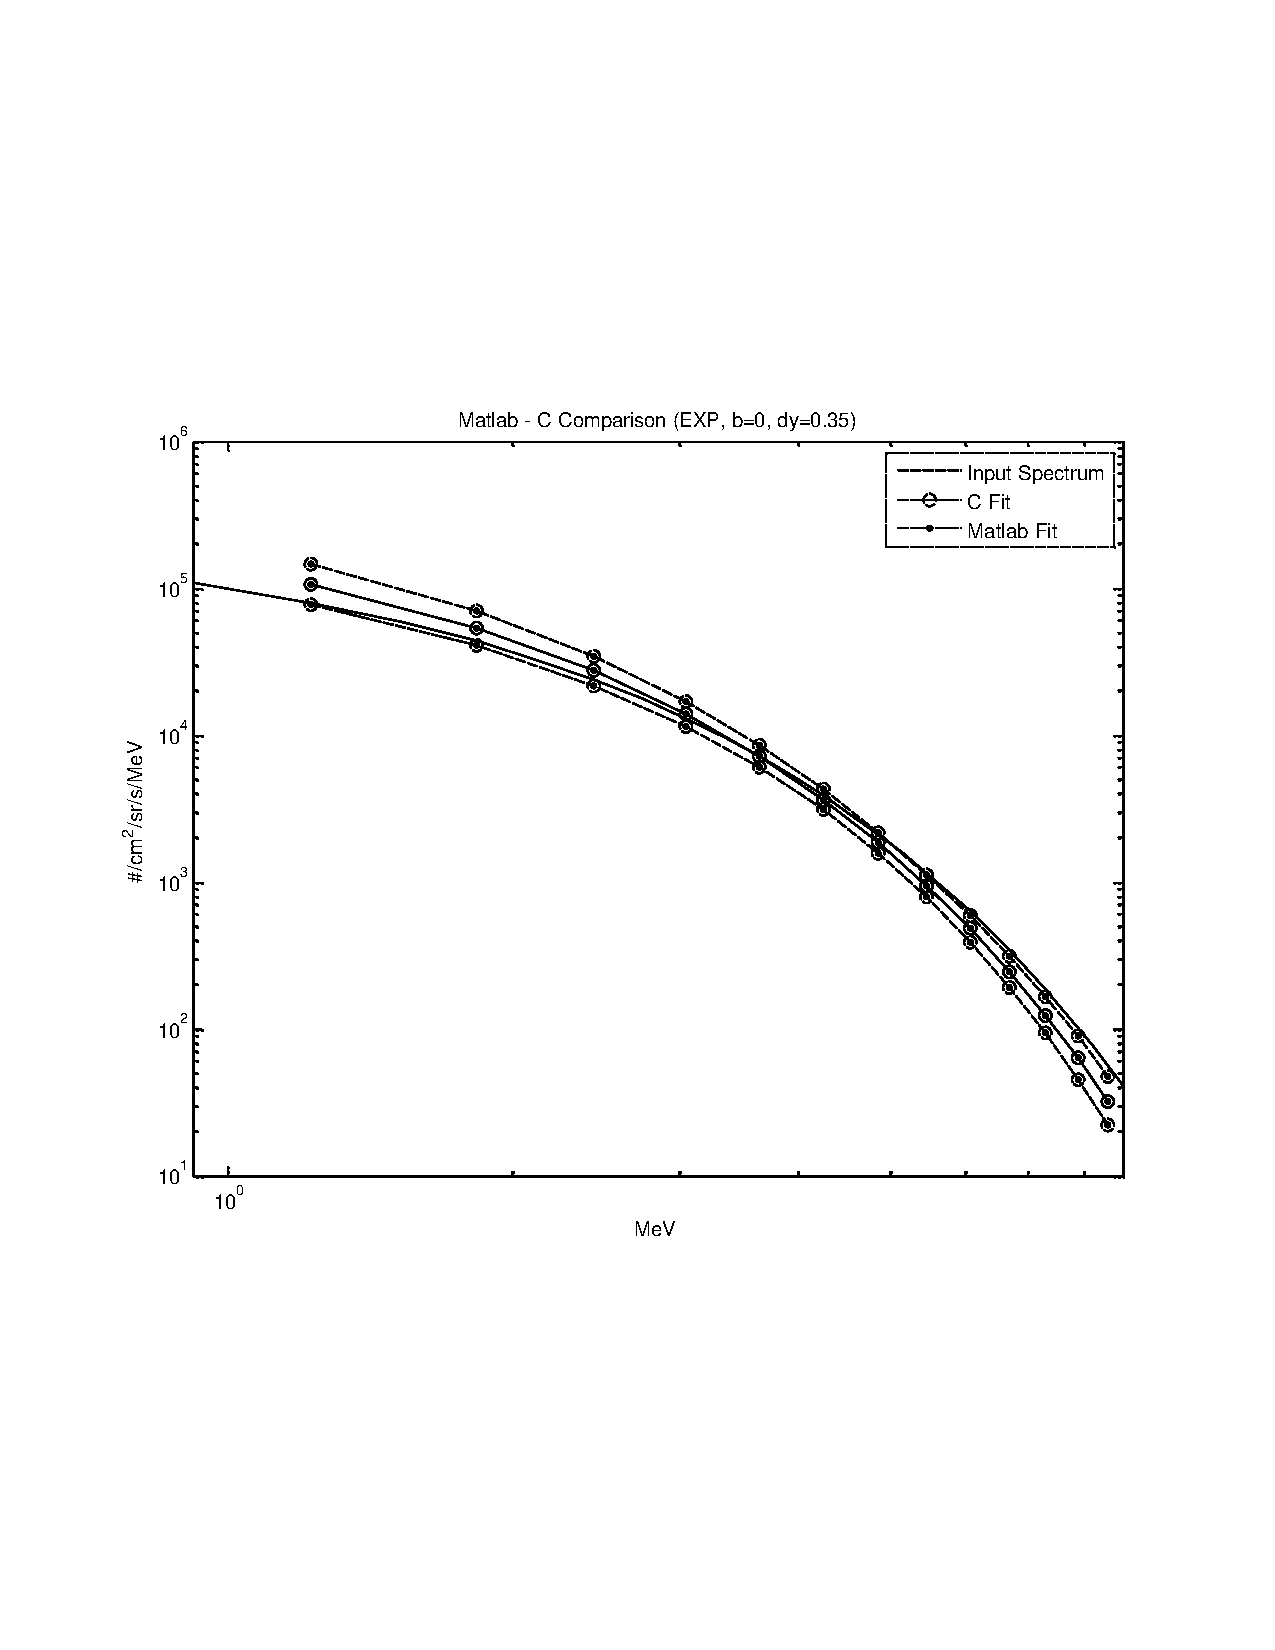
\includegraphics[width=40pc]{ana_spec_inv_MatlabC.pdf}
}
\caption{An example of fitting power law (PL) and exponential (EXP) spectra
  to the counts in 5 ICO electron channels to a simulated exponential
  with Poisson noise. Dotted lines indicate 1 standard error above and
  below the fits.}
\label{figAnalyticalFitExample}
\end{figure}

Validation has consisted of validation of individual ``private''
routines found in the various `.c'' files but not shared via
``invlib.h'', as well as the shared \verb|ana_spec_inv routine|. The C
and Matlab codes agree to within 5 or 6 decimal places for inputs of
noisy power-law and exponential distributions fit to combinations of
power-law, exponential and relativistic Maxwellian spectra.

\subsection{Library Function ana\_spec\_inv\_multi}
The library also provides a multi-case function,
\verb|ana_spec_inv_multi|, with the following C prototype (found in
``invlib.h''):
\begin{verbatim}
int ana_spec_inv_multi(const long int Ntimes,
		       const double *y, const double *dy, 
		       const double *Egrid, const double *H0, 
		       const double *dt, const double *b,
		       const long int *int_params, const double *real_params,
		       char *outFile, double *Eout, 
		       double *flux, double *dlogflux, 
		       double *lambda, double *support_data, 
		       int *result_codes);
\end{verbatim}
This function calls \verb|ana_spec_inv| \verb|Ntimes|, in each case
advancing the \verb|y| and \verb|b| pointers by \verb|NY| (i.e.,
moving one row forward, if \verb|y| and \verb|b| are interpreted as
\verb|Ntimes|$\times$\verb|NY| row-major matrices), and, similarly,
advancing \verb|flux| and \verb|dlogflux| by
\verb|NE|. \verb|lambda| is advanced by \verb|NY|.
\verb|support_data| is advanced by $(2+\verb|ASI_MAX_NQ|+\verb|NY|)\times(\verb|ASI_MAX_POW2|+1)$,
where \verb|ASI_MAX_POW2| is presently 4 since $2^4$ is the largest
function bitmap value, and is defined in ``specinv.h'' for C users.

\verb|result_codes| provides the functional return values.
The primary difference between \verb|ana_spec_inv| and
\verb|ana_spec_inv_multi| is that the latter requires
the aggregation time (\verb|dt|) be passed in separately from the
instrument response function. For each call to \verb|ana_spec_inv|, a
temporary \verb|H| will be set to \verb|H0|$\times$\verb|dt[t]|, to
reflect a possibly changing integration time. The other inputs
are passed directly to \verb|ana_spec_inv|, without alteration.

The return code of \verb|ana_spec_inv_multi| is typically the first
non-success result code returned by the multiple calls
\verb|ana_spec_inv|. Of course, if all calls to \verb|ana_spec_inv| succeed,
the return code from \verb|ana_spec_inv_multi| will indicate
success. The only additional exception is if \verb|Ntimes|$<1$, in
which case the empty input array error code will be returned (-102).


\section{Library Functions omni2uni and wide2uni}

This section describes planned angular inversion functions for
single-channel omnidirectional and wide-angle measurements.

The following C prototypes will be added to ``invlib.h'':
\begin{verbatim}
int omni2uni(const double *omniflux, const double *dlogomniflux,
             const long int *int_params, 
             const double *real_params,
             char *outFile, 
             double *uniflux, double *dloguniflux);
\end{verbatim}

\begin{verbatim}
int wide2uni(const double *wideflux, const double *dlogwideflux,
             const double *PAgrid, const double *H, 
             const long int *int_params, 
             const double *real_params,
             char *outFile,
             const long int *ialpha0,
             double *uniflux, double *dloguniflux);
\end{verbatim}
Returns estimated flux at \verb|PAgrid[ialpha0]|, where \verb|H|
describes angular dependence on grid \verb|PAgrid|.

\subsection{Calculations Performed - TEM-1 Method}

The omnidirectional or wide-angle flux is given by:
\begin{equation}
f_{\rm iso} = \int_0^{2\pi} \int_0^{\pi} h(\alpha,\phi) f_{\rm uni}(\alpha) \sin\alpha d\alpha d\phi.
\end{equation}
We denote the wide-angle or omnidirectional flux $f_{\rm iso}$ under
the assumption that \verb|wideflux| or \verb|omniflux| is given in
the form of a isotropic unidirectional flux (e.g., \#/cm$^2$/s/sr/keV).
For the wide-angle approximation, one has a bit more flexibility: it
is only necessary to provide \verb|H| and \verb|wideflux| in
appropriate units so that the units of \verb|uniflux| will be the
units of \verb|wideflux| divided by the units of \verb|H|.

The omnidirectional flux is a special case of the wide-angle flux problem:
\begin{equation}
h(\alpha,\phi) = \frac{1}{4\pi}.
\end{equation}

First, we discretize this equation:
\begin{eqnarray}
f_{\rm iso} &\approx& \sum_i H_i f_i, \\ 
H_i &\approx& \int_0^{2\pi} h(\alpha_i,\phi) d\phi \sin\alpha_i \Delta\alpha_i, \\
f_i &=& f_{\rm uni}(\alpha_i).
\end{eqnarray}

TEM-1 follows Vette's AE-8 atmospheric cutoff:
\begin{eqnarray}
\frac{B_m}{B_0} = \left\{
\begin{array}{cl}
0.6572 L_m^{3.452} & L_m < 2.4 \\
0.196 L_m^{4.878} & 2.4 \le L_m < 3.0 \\
1.4567 L_m^{3.050} & L_m >3.0 \\
\end{array}
\right.
\end{eqnarray}
Any flux outside (i.e., with $B_m/B_0$ beyond the limit) is treated as
implicitly zero by removing it from the $\vec{f}$.  By implication,
there is no electron flux at any pitch angle for $L_m < 1.1293$.
Requesting a unidirectional flux at a local pitch angle that mirrors
beyond the cutoff will result in an error code (see Return Codes,
section \ref{secTEM1retcodes}).

Next, we set the problem up as a constrained maximum likelihood equation in the log fluxes:
\begin{eqnarray}
x_i &=& \ln f_i, \\
y &=& \verb|wideflux|, \\
\delta y &=& \verb|dlogwideflux|, \\
\lambda &=& \sum_i H_i f_i, \\
\ell &=& \Lambda(\ln\lambda-\ln y) + \frac{1}{2}(\vec{x}-\vec{\mu})^T \dbul{\Sigma}^{-1} (\vec{x}-\vec{\mu}). \label{eqTEM1ell}
\end{eqnarray}
The LaGrange multiplier $\Lambda$ ensures that the local minimum in
$\ell$ satisfies $y=\lambda$, i.e., the inverted angular distribution
exactly reconstructs the observed wide-angle flux. 

Note: I also tried using a typical log-normal penalty function on $y$
based on $\delta y$, but that approach causes the solution $\vec{x}$
to be systematically biased toward $\vec{\mu}$. This is a typical
problem with maximum likelihood. I believe we ought to treat
separately the uncertainty in the wide-angle measurement and the
uncertainty in the conversion to unidirectional flux. This LaGrange
multiplier approach does just that.

The second term in (\ref{eqTEM1ell}) is the likelihood of a particular
local pitch angle distribution at the specified energy and location
according to TEM1. TEM1 provides the median $m_{50}(E,\alpha_eq,L_m)$,
95$^{\rm th}$ percentile $m_{95}(E,\alpha_eq,L_m)$, and spatial
correlation coefficient $\rho(\alpha_{eq,i},\alpha_{eq,i'}|E,L_m)$,
and we can convert between $\alpha$ and $\alpha_{eq}$ using the
$B/B_0$ parameter.

\begin{eqnarray}
\sin\alpha_{eq,i} &=& \frac{\sin\alpha_i}{\sqrt{B/B_0}}, \\
\mu_i &=& \ln m_{50}(E,\alpha_{eq,i},L_m), \\
\sigma_i &=& (\ln m_{95}(E,\alpha_{eq,i},L_m)-\mu)/\Phi^{-1}(0.95), \\
\Phi^{-1}(0.95) &=& 1.6448536270, \\
\Sigma_{ii'} &=& \sigma_i \sigma_{i'} \rho(\alpha_{eq,i},\alpha_{eq,i'}|E,L_m).
\end{eqnarray}

To solve for $\ell$ will require the usual gradients and derivatives:
\begin{eqnarray}
\frac{\partial \lambda}{\partial x_i} &=& H_i f_i\\
\frac{\partial \ell}{\partial x_i} &=&
(\Lambda/\lambda) H_i f_i + \sum_{i'}\left(\dbul{\Sigma}^{-1}\right)_{ii'}(x_{i'}-\mu_{i'}) , \label{eqGradEllx} \\
\frac{\partial \ell}{\partial \Lambda} &=& \ln\lambda-\ln y, \label{eqGradEllLambda} \\
\frac{\partial^2 \ell}{\partial x_i \partial x_{i'}} &=&
(\Lambda/\lambda) H_i f_i \delta_{ii'} 
-(\Lambda/\lambda^2) H_i f_i H_{i'} f_{i'} +
\left(\dbul{\Sigma}^{-1}\right)_{ii'}, \\
\frac{\partial^2 \ell}{\partial x_i \partial \Lambda} &=&
H_i f_i/\lambda, \\
\frac{\partial^2 \ell}{\partial \Lambda^2} &=& 0.
\end{eqnarray}

The initial guess is $y/(\vec{H}^T\exp(\vec{\mu}))$, i.e., the median
fluxes are rescaled to reconstruct $y$.  The fit for $\vec{x}$ is
performed with multivariate root finding routines provided by the Gnu
Scientific Library, producing the maximum likelihood value
$(\hat{\vec{x}}^T,\hat{\Lambda})$, which finds simultaneous zeros of (\ref{eqGradEllx})
and (\ref{eqGradEllLambda}).

Thus the estimated flux is:
\begin{equation}
\verb|uniflux| = \exp(\hat{x}_{i_{\alpha_0}}).
\end{equation}
We discard all the other components of $\hat{\vec{x}}$ because we want
to conserve the number of observations (one cannot get something for
nothing) for subsequent analysis. Doing otherwise would risk
over-weighting the ``typical'' pitch angle distribution shape in
subsequent analysis of the inverted flux.

The uncertainty on the log flux is given by:
\begin{eqnarray}
\verb|dloguniflux| &=& 
\sqrt{(\delta y)^2 + (\delta \ln f_{i_{\alpha_0}} )^2}, \\
\delta\ln f_{i_{\alpha_0}} &=& \delta x_{i_{\alpha_0}} =
\sqrt{Q_{i_{\alpha_0},i_{\alpha_0}}}, 
\\
\dbul{Q} &=& \left(
  \begin{array}{cc}
  \begin{array}{ccc}
    ~ & \vdots & ~ \\
    \cdots & \left.
      \frac{\partial^2 \ell}{\partial x_i \partial x_{i'}}\right|_{(\hat{\vec{x}}^T,\hat{\Lambda})}
    & \cdots \\
    ~ & \vdots & ~ 
  \end{array} & \left.\frac{\partial \ell}{\partial \Lambda}\right|_{(\hat{\vec{x}}^T,\hat{\Lambda})} \\
  \left.\frac{\partial \ell}{\partial \Lambda}\right|_{(\hat{\vec{x}}^T,\hat{\Lambda})} & 0
  \end{array}
\right)^{-1}.
\end{eqnarray}
Note that $\dbul{Q}$ is the inverse of the Hessian of $\ell$ in the
$(\vec{x}^T,\Lambda)$ super-space, and \verb|dloguniflux| is a
combination of the angular inversion error and the measurement error
\verb|dlogwideflux|, as if they were independent (not a bad
assumption).

\subsection{Calculations Performed - Vampola Method}

The Vampola method is based on a $\sin^n\alpha$ fit, where $n$ depends
on the $L$ shell, in this case McIlwain $L_m$ in Olson-Pfitzer
Quiet. Table~\ref{tblVampola} gives the coefficients provided in
\citet{Vampola1996}. For $L_m$ in bounds, linear interpolation
is used. For $L_m$ out of bounds, the nearest boundary value is used.

\begin{table}[htbp]
\caption{Exponent in $\sin^n\alpha$ fits from \citet{Vampola1996}}
\label{tblVampola}
\begin{tabular}{ll}
$L_m$ & $n$ \\
\hline
    3.00 &   5.380 \\
    3.25 &   5.078 \\
    3.50 &   4.669 \\
    3.75 &   3.916 \\
    4.00 &   3.095 \\
    4.25 &   2.494 \\
    4.50 &   2.151 \\
    4.75 &   1.998 \\
    5.00 &   1.899 \\
    5.25 &   1.942 \\
    5.50 &   1.974 \\
    5.75 &   1.939 \\
    6.00 &   1.970 \\
    6.25 &   2.136 \\
    6.50 &   1.775 \\
    6.75 &   1.438 \\
    7.00 &   1.254 \\
    7.25 &   1.194 \\
    7.50 &   1.046 \\
    7.75 &   0.989 \\
    8.00 &   0.852
\end{tabular}
\end{table}

Whereas the TEM-1 method required a constrained minimization, the
Vampola method requires only a numerical integral:

\begin{eqnarray}
f_{\rm uni}(\alpha) &=& f_0 \sin^n\alpha, \\
f_{\rm iso} &\approx& \sum_j H_j f_0 \sin^n \alpha_j , \\ 
\verb|uniflux| &=& \frac{f_{\rm iso}}{\sum_{j} H_j f_0 \sin^n \alpha_j}\sin^n\alpha_{0}.
\end{eqnarray}

The Vampola method also uses the AE8 atmospheric cutoff, like TEM-1.
Finally, because Vampola did not provide error estimates on $n$, the
output error estimate (\verb|dloguniflux|) for the Vampola method is
the input error (\verb|dlogomniflux| or \verb|dlogwideflux|).


\subsection{Function Arguments}

\subsubsection{omni2uni}
\begin{itemize}
\item \verb|omniflux|  (input) Estimated isotropic unidirectional flux (for TEM-1 method, use \#/cm$^2$/sr/s/keV).
\item \verb|dlogomniflux| (input) relative error for \verb|omniflux| (dimensionless).
\item \verb|int_params| (input) integer parameters, length = 5 (TBR).
\subitem \verb|int_params[0]| \verb|NA| = number of grid points for angular integral.
\subitem \verb|int_params[1]| angular inversion method:
\subsubitem[-1] - TEM-1.
\subsubitem[-2] - Vampola.
\subitem \verb|int_params[2]| Verbose setting (choose one):
\subitem \verb|int_params[3]| Choice of root finder (choose one):
\subsubitem[0] Powell's Hybrid method, scaled (recommended),
\subsubitem[1] Powell's Hybrid method
\subsubitem[2] Newton's method
\subsubitem[3] Pseudo-global Newton's method
\subsubitem[4] Powell's Hybrid method w/ numerical Hessian, scaled
\subsubitem[5] Powell's Hybrid method w/ numerical Hessian
\subsubitem[6] Discrete Newton's method  (numerical Hessian)
\subsubitem[7] Broyden's algorithm (numerical Hessian)
\subitem \verb|int_params[4]| Maximum number of iterations by minimizer (recommend 10,000).
\subsubitem[0] no text output,
\subsubitem[1] text output to standard output stream,
\subsubitem[2] text output to standard error stream,
\subsubitem[3] text output to outFile (assumes outFile is actually a \verb|FILE *|).
\subsubitem[4] text output to outFile, overwrite existing file
\subsubitem[5] text output to outFile, append to existing file
\item \verb|real_params| (input) real parameters, length 3 (TBR).
\subitem \verb|real_params[0]| = Energy of electron flux energy, keV
\subitem \verb|real_params[1]| = $B/B_0$ of spacecraft location, dimensionless.
\subitem \verb|real_params[2]| = $L_m$, McIlwain L for locally mirroring electron, in Olson-Pfitzer Quiet.
\item \verb|outFile| (input) provides filename or \verb|FILE *| for verbose output (see verbose setting above). Null terminated string.
\item \verb|uniflux| (output) Locally-mirroring unidirectional flux, (e.g., in \#/keV/cm$^2$/sr/s).
\item \verb|dloguniflux| (output) Standard error of natural log of \verb|uniflux| (dimensionless).
\end{itemize}

\subsubsection{wide2uni}
\begin{itemize}
\item \verb|wideflux|  (input) Estimated isotropic unidirectional flux  (for TEM-1 method, use \#/cm$^2$/sr/s/keV).
\item \verb|dlogwideflux| (input) relative error for \verb|wideflux| (dimensionless).
\item \verb|PAgrid| (input) \verb|PAgrid[i]| local pitch angle at grid point $i$, degrees, must be monotonically increasing grid.
\item \verb|H| (input) \verb|H[i]| Angular weighting for unidirectional flux at grid point $i$, dimensionless.
\item \verb|int_params| (input) integer parameters, length = 5 (TBR), same as \verb|omni2uni| except:
\subsubitem[0] = \verb|NA| number of pitch angles in grid.
\item \verb|real_params| (input) same as \verb|omni2uni|.
\item \verb|outFile| (input) same as \verb|omni2uni|.
\item \verb|ialpha0| (input) zero-based index of pitch angle grid point for uniflux output (e.g., grid point nearest sensor bore sight).
\item \verb|uniflux| (output) same as \verb|omni2uni|.
\item \verb|dloguniflux| (output) same as \verb|omni2uni|.
\end{itemize}

Notes: 
\begin{enumerate}
\item Pointers are used throughout for ease of access from FORTRAN, which can only pass arguments by reference (i.e., pointers).
\item Array and matrix indices above are zero-based, following C convention rather than one-based linear algebra convention.
\item \verb|omni2uni| and \verb|wide2uni| operate on estimated isotropic unidirectional flux.
\item Alternatively, \verb|H| and \verb|wideflux| can be defined in terms of omnidirectional flux, so long as
the units of \verb|wideflux|/\verb|H| give units of \verb|uniflux|.
\item If \verb|dlogomniflux| or \verb|dlogwideflux| is unknown, use $\ln(2)/2$ for factor of 2 95\% confidence bounds.
\item \verb|omniflux|, \verb|wideflux|, \verb|dlogomniflux|, or
  \verb|dlogwideflux| negative or zero will result in an error (see
  Return Codes, section \ref{secTEM1retcodes}).
\item \verb|outFile| is ignored for verbose settings 0, 1, and 2.
\item The 95\% confidence interval on \verb|uniflux| is given by $\verb|uniflux|\times\exp(\pm 1.9600\times\verb|dloguniflux|)$.
\end{enumerate}

\subsection{Return Codes}
\label{secTEM1retcodes}
\begin{itemize}
\item[1] Success! No Error.
\item[0] Unknown error (this only happens if there's a bug).
\item[-101] NULL passed where pointer expected.
\item[-102] One or fewer valid data points (\verb|NY|$ \le 1$), or \verb|NE|$\le 1$ or \verb|NEout|$<1$.
\item[-103] One or more invalid (NaN or infinite) in input arrays, or 
  some \verb|y[i]|$<0$, \verb|dy[i]|$<0$, \verb|Egrid[j]|$\le 0$, or \verb|Egrid[j]|$\le 0$.
\item[-104] Negative or zero input \verb|omniflux|, \verb|wideflux|, \verb|dlogomniflux|, \verb|dlogwideflux|.
\item[-401] Invalid minimizer selected.
\item[-402] Invalid iterations requested (zero or negative).
\item[-501] Invalid value of verbose provided or user-requested file stream NULL (outFile).
\item[-502] User-requested verbose output file (outFile) could not be opened.
\item[-601] Output pitch angle requested out of range (index out of range or $B_m$ beyond cutoff).
\item[-602] Invalid angular inversion method requested.
\end{itemize}

\subsection{Validation}

The routine \verb|omni2uni| has been validated for the TEM-1 method by
running it for various cases and examining the output for sanity (not
very sophisticated validation). The C test code is is
``omni2uni\_test.c'', which passes a single test case to
\verb|omni2uni| and prints it output.

Here is a transcript of \verb|omni2uni_test.exe|:
\begin{verbatim}
[PROMPT]> ./omni2uni_test.exe
omni2uni_test:inputs = omni=1.00000e+04 (dlog=3.46574e-01) @ [300.0 keV, B/B0=400.00, Lm=6.60]
fzero Invoked with solver hybridsj, MaxIter=1000
fzero: 1/1000: 0.313671:
fzero: 2/1000: 0.0140756:
fzero: 3/1000: 1.27369e-06:
fzero: 4/1000: 3.37084e-09:
fzero: completed after 4/1000: success
omni2uni_test:inputs = omni=1.00000e+04 (dlog=3.46574e-01) @ [300.0 keV, B/B0=400.00, Lm=6.60]
omni2uni_test:result = 1, uni=2.73852e+04 (dlog=3.46656e-01)
[PROMPT]> 
\end{verbatim}
In this case, because $B/B0>>1$, there is a substantial loss cone,
thus creating a significant pitch-angle anisotropy, which results in a
much larger locally-mirroring flux than would be assumed from isotropy
alone (by a factor of 2.7...).

\section{Dependencies and Compiling}

The inversion library routines rely on the GNU Scientific Library,
available for free download at http://www.gnu.org/software/gsl/. The
GSL base library and the GSL CBLAS library are required (both come
with a typical GSL install).

The library is built for the gcc compiler suite. A makefile
(``Makefile'') is provided. The \verb|make| command alone will display
the helps required to build the \verb|invlib| shared object (DLL).

The compilation may generate some \verb|warning| and \verb|Info| messages:
\begin{verbatim}
warning: comparison between signed and unsigned
warning: assignment discards qualifiers from pointer target type
Info: resolving _gsl_multimin_fdfminimizer_conjugate_fr by linking to
 __imp__gsl_multimin_fdfminimizer_conjugate_fr (auto-import)
Info: resolving _gsl_multimin_fdfminimizer_conjugate_pr by linking to
 __imp__gsl_multimin_fdfminimizer_conjugate_pr (auto-import)
Info: resolving _gsl_multimin_fminimizer_nmsimplex by linking to
 __imp__gsl_multimin_fminimizer_nmsimplex (auto-import)
Info: resolving _gsl_multimin_fdfminimizer_vector_bfgs2 by linking to
 __imp__gsl_multimin_fdfminimizer_vector_bfgs2 (auto-import)
\end{verbatim}

I have not figured out how to make a stand-alone DLL in cygwin, I
think because GSL libraries depend on ``cygwin1.dll''. However, I have
created a DLL with MSYS/MINGW, and the makefile has commands to do
this.


\appendix
\section{Adding a new spectral form}
\label{secAddingSpectrum}

The following modifications must be made to add a new spectral form:

In \verb|specinv.h|, 
\begin{itemize}
\item add a new \verb|ASI_FXN_<NEW>| constant, the next power of two.
\item increment \verb|ASI_FXN_POW2| constant,
\item insert \verb|ASI_FXN_<NEW>| in bitwise or of all allowed functions (\verb|ASI_FXN_ALL|)
\end{itemize}

In \verb|invlib_const.h|, add any new error codes associated with
improper options/settings for new analytical spectrum.

In \verb|specinv.c|, 
\begin{itemize}
\item create new \verb|flux_<new>| function, following template from existing analytical flux functions.
\item add input checks to \verb|ana_spec_inv|, e.g., checking for existence and positivity of rest mass parameter in \verb|params|.
\item add case for \verb|ASI_FXN_<NEW>| to \verb|switch(fxn_bit)| in \verb|ana_spec_inv|.
\end{itemize}

In \verb|invlib.tex| (this file), add appropriate documentation:
\begin{itemize}
\item Note changes in section \ref{secChanges}, ``Changes''.
\item Add definition and derivatives of new spectral function to section \ref{secAnalyticalSpectra}.
\item Update argument list for \verb|ana_spec_inv|, section \ref{secAnaSpecInvArgs}.
\end{itemize}

Test compilation with \verb|make| commands. Recompile this file with \verb|pdflatex|.

\begin{thebibliography}{}
\bibitem[{\it Vampola}(1996)]{Vampola1996}
Vampola, A.L.
Outer zone energetic electron environment update,
{\it Final Report of ESA/ESTEC/WMA/P.O. 151351}, 
ESA-ESTEC, Noordwijk, The Netherlands, 1996.
\end{thebibliography}


\end{document}             % End of document.

